
%%%%%%%%%%%%%%%%%%%%%%% file typeinst.tex %%%%%%%%%%%%%%%%%%%%%%%%%
%
% This is the LaTeX source for the instructions to authors using
% the LaTeX document class 'llncs.cls' for contributions to
% the Lecture Notes in Computer Sciences series.
% http://www.springer.com/lncs       Springer Heidelberg 2006/05/04
%
% It may be used as a template for your own input - copy it
% to a new file with a new name and use it as the basis
% for your article.
%
% NB: the document class 'llncs' has its own and detailed documentation, see
% ftp://ftp.springer.de/data/pubftp/pub/tex/latex/llncs/latex2e/llncsdoc.pdf
%
%%%%%%%%%%%%%%%%%%%%%%%%%%%%%%%%%%%%%%%%%%%%%%%%%%%%%%%%%%%%%%%%%%%


\documentclass[runningheads,a4paper]{llncs}

\usepackage{amssymb}
\setcounter{tocdepth}{3}
\usepackage{graphicx}

\usepackage{url}
\urldef{\mailsa}\path|{yingqin,syshen,|
\urldef{\mailsb}\path|huadongdai,|
\urldef{\mailsc}\path|qingbowu,yanjia}@nudt.edu.cn|
\newcommand{\keywords}[1]{\par\addvspace\baselineskip
\noindent\keywordname\enspace\ignorespaces#1}

\newtheorem{algorithm}{Algorithm}

\begin{document}

\mainmatter  % start of an individual contribution

% first the title is needed
%\title{Lecture Notes in Computer Science:\\Authors' Instructions
%for the Preparation\\of Camera-Ready
%Contributions\\to LNCS/LNAI/LNBI Proceedings}
\title{Complementary Synthesis for Encoders with Pipeline and Flow Control Mechanism}

% a short form should be given in case it is too long for the running head
%\titlerunning{Lecture Notes in Computer Science: Authors' Instructions}

% the name(s) of the author(s) follow(s) next
%
% NB: Chinese authors should write their first names(s) in front of
% their surnames. This ensures that the names appear correctly in
% the running heads and the author index.
%
\author{Ying Qin %
%\thanks{Project 61070132 supported by National Natural Science Foundation of China.}%
\and ShengYu Shen \and HuaDong Dai \and QingBo Wu \and Yan Jia}
%
\authorrunning{Ying Qin %
\and ShengYu Shen \and HuaDong Dai \and QingBo Wu \and Yan Jia}
% (feature abused for this document to repeat the title also on left hand pages)

% the affiliations are given next; don't give your e-mail address
% unless you accept that it will be published
\institute{School of Computer, National University of Defense Technology, China\\
\mailsa\mailsb\mailsc\\
% \url{}
}

%
% NB: a more complex sample for affiliations and the mapping to the
% corresponding authors can be found in the file "llncs.dem"
% (search for the string "\mainmatter" where a contribution starts).
% "llncs.dem" accompanies the document class "llncs.cls".
%

\toctitle{Lecture Notes in Computer Science}
\tocauthor{Authors' Instructions}
\maketitle


\begin{abstract}
Complementary synthesis automatically generates an encoder's decoder
that recovers the encoder's inputs from its output,
even if this encoder contains flow control mechanism that prevents
its inputs from being uniquely determined by its outputs.
At the same time,
most encoders also include pipeline stages to improving timing.
Such a structure can be exploited to also improve the decoder's timing.
\vspace{0.1cm}

This paper proposes a novel algorithm to handle encoders with both pipeline and flow control mechanism.
First,
it infers the flow control predicate on inputs with state-of-the-art algorithm.
Second,
it finds out the pipeline stages in the encoder by enforcing the inferred flow control predicate.
Third,
it infers the flow control predicate for each pipeline stages.
Finally,
the decoder's Boolean functions that recover each pipeline stage and input are characterized with Craig interpolant.

\vspace{0.1cm}

Experimental results on several complex encoders indicate that
this algorithm can always correctly generate a pipelined decoders with inferred flow control mechanism.

\keywords{Complementary Synthesis, Flow Control Mechanism, Pipeline Stage, Craig Interpolation}
\end{abstract}


\section{Introduction}\label{sec_intro}
One of the most difficult jobs in designing communication
and multimedia chips is to design and verify complex encoder and decoder pairs.
The encoder maps its input variables $\vec{i}$ to its output variables $\vec{o}$,
% according to some predefined rules,
% such as Ethernet \cite{IEEE8023_S4} and PCI Express \cite{pcie21},
while the decoder recovers $\vec{i}$ from $\vec{o}$.
Complementary synthesis 
\cite{ShenICCAD09,ShenTCAD11,ShenTCAD12,LiuICCAD11,LiuTCAD12,TuDAC13}
eases this job by
automatically generating a decoder from an encoder,
with the assumption that $\vec{i}$ can always be
uniquely determined by a bounded sequence of $\vec{o}$.
Thus,
the decoder's Boolean function can be characterized
with the algorithm proposed by Jiang et al. \cite{InterpBoolFunction}
This algorithm constructs an unsatisfiable formula with two unrolled transition function sequences,
both of which have the same output sequence but with different input.
A Craig interpolant \cite{Craig} can be extracted from this unsatisfiable formula,
and used as the decoder's Boolean function that recovers the inputs.

However,
the flow control mechanism widely employed in encoders of modern communication protocols
fails this simple assumption.
To prevent the faster transmitter from overwhelming slower receiver,
when the receiver can't keep up with the transmitter,
flow control mechanism \cite{flowcontrol} will not transmit valid data symbols,
but instead transmit idle symbols that can only uniquely determine a small subset of inputs.
We call such inputs the flow control vector $\vec{f}$,
and other inputs the data vector $\vec{d}$.
Qin et al. \cite{QinTODAES15} handle such encoders by
first finding out all inputs $i\in\vec{i}$ that can by uniquely determined by $\vec{o}$,
and taking them as $\vec{f}$,
and then inferring a predicate $valid{\vec{f}}$ that,
when enforced,
can make $\vec{d}$ to be uniquely determined by $\vec{o}$.


At the same time,
in almost all modern encoders circuits,
pipeline stages are inserted to cut the datapath into multiple segments,
such that the encoder can run in higher frequency.
But the flow controlled decoder generated by \cite{QinTODAES15} does not include pipeline stages,
which make it much slower than the corresponding encoder.

To overcome this problem,
this paper proposes a novel algorithm to generate pipelined decoders for flow controlled encoder.
It first apply Qin et al. \cite{QinTODAES15}'s algorithm to find out $\vec{f}$ and infers $valid(\vec{f})$ that can make $\vec{d}$ to be uniquely 
determined by $\vec{o}$.
It then finds out the pipeline stages $\vec{stg}^j$ in the encoder by enforcing $valid(\vec{f})$.
and infers the flow control predicates $valid^j(\vec{stg}^j)$ for each pipeline stage.
It finally characterize the Boolean function that recover each $\vec{stg}^j$ and $\vec{i}$ with 
Jiang et al. \cite{InterpBoolFunction}'s algorithm.

\emph{The remainder of this paper is organized as follows}.
%Section \ref{sec_casestudy} explains our ideas with a simple example.
Section \ref{sec_prem} introduces the background material;
Section \ref{sec_findfc} identifies the flow control variables,
and infers the predicate that enables $\vec{d}$ 
to be uniquely determined by a bounded sequence of $\vec{o}$;
Section \ref{sec_pipe} infers the pipeline stages $\vec{stg}^j$,
while Section \ref{sec_pred} infers  $valid^j(\vec{stg}^j)$ for each pipeline stage;
Sections \ref{sec_exp} and \ref{sec_relwork} present the experimental results and related works;
Finally,
Section \ref{sec_conclude} sums up the conclusion.

\section{Preliminaries}\label{sec_prem}

% \subsection{Flow control mechanism}\label{subsec_fc}



\subsection{Propositional satisfiability}\label{subsec_SAT}
% We use a denotation similar to that of \cite{TuDAC13}.
The Boolean value set is denoted as $B=\{0,1\}$.
A vector of variables is represented as $\vec{v}=(v,\dots)$.
The number of variables in $\vec{v}$ is denoted as $|\vec{v}|$.
If a variable $v$ is a member of $\vec{v}$,
% that is $\vec{v}=(\dots,v,\dots)$,
then we say $v\in\vec{v}$;
otherwise we say $v\notin\vec{v}$.
For a variable $v$ and a vector $\vec{v}$,
if $v\notin\vec{v}$,
then the new vector that contains both $v$ and all members of $\vec{v}$ is denoted as $v\cup\vec{v}$.
If $v\in \vec{v}$,
then the new vector that contains all members of $\vec{v}$ except $v$,
is denoted as $\vec{v}-v$.
For the two vectors $\vec{a}$ and $\vec{b}$,
the new vector with all members of $\vec{a}$ and $\vec{b}$ is denoted as $\vec{a}\cup\vec{b}$.
The set of truth valuations of $\vec{v}$ is denoted as $[\![\vec{v}]\!]$,
for instance,
$[\![(v_1,v_2)]\!]=\{(0,0),(0,1),(1,0),(1,1)\}$.

A Boolean formula $F$ over a variable set $V$ is constructed by connecting variables from $V$ 
with symbols $\neg$, $\wedge$, $\vee$ and $\Rightarrow$,
which stand for logical connectives negation, conjunction, disjunction, and implication, respectively.

The propositional satisfiability problem(abbreviated as SAT) for a Boolean formula $F$ over a variable set $V$ 
is to find a satisfying assignment $A:V\to B$,
so that $F$ can be evaluated to $1$.
If $A$ exists, then $F$ is satisfiable;
otherwise,
it is unsatisfiable.

% A computer program that decides the existence of such a satisfying assignment is called a SAT solver,
%  such as Zchaff\cite{CHAFF},
%  Grasp\cite{grasp},
%  Berkmin\cite{BERKMIN},
%  and MiniSat\cite{EXTSAT}.
 
% Normally,
% a SAT solver requires the formula to be represented in the conjunctive normal form(CNF),
% in which a formula is a conjunction of its clause set,
% and a clause is a disjunction of its literal set,
% and a literal is a variable or its negation.
% A formula in the CNF format is also called a SAT instance,


% \subsection{Cofactoring}\label{subsec_pre_cofact}

% For a Boolean function $f:B^n\to B$,
% we use $supp(f)$ to denote its support set $\{v_1\dots v_n\}$.
According to \cite{EFFSATUSMCCO},
the positive and negative cofactors of $f(v_1\dots v\dots v_n)$ with respect to variable
$v$ are $f_{v\equiv 1}=f(v_1\dots 1\dots v_n)$ and $f_{v\equiv 0}=f(v_1\dots 0\dots v_n)$,
respectively.
% Existential quantification of $f(v_1\dots v\dots v_n)$ with respect to a
% variable $v$ is $\exists v f=f_v+f_v’$.
\textbf{Cofactoring} is the action that applies 1 or 0 to $v$ to get $f_{v\equiv 1}$ or $f_{v\equiv 0}$.

% \subsection{Craig interpolation}\label{subsec_pre_interp}
% Craig\cite{Craig} had proved the following theorem:
% \begin{theorem}[Craig Interpolation Theorem\cite{Craig}]\label{thm_craig}
Given two Boolean formulas $\phi_A$ and $\phi_B$,
with $\phi_A\wedge \phi_B$ unsatisfiable,
there exists a formula $\phi_I$ referring only
to the common variables of $\phi_A$ and $\phi_B$ such that $\phi_A\Rightarrow \phi_I$
and $\phi_I\wedge \phi_B$ is unsatisfiable.
We call $\phi_I$ the \textbf{interpolant} \cite{Craig} of $\phi_A$ with respect to $\phi_B$
% \end{theorem}
and use McMillan's algorithm \cite{interp_McMillan} to generate it.

% In the remainder of this paper,
% we will focus on the propositional logic only,
% There are many approaches to generate interpolants for propositional logic,
% so please refer to Krajicek\cite{interp_Krajicek},
% Pudlak\cite{interp_Pudlak} and McMillan\cite{interp_McMillan} for more details.
% which is generated by MiniSat\cite{EXTSAT}.


% \subsection{Incremental SAT mechanism of MiniSat solver}\label{subsec_incsat}

% In this paper,
MiniSat \cite{EXTSAT} is used in this paper to solve all formulas.
% Like many other SAT solver based on conflict driven learning \cite{CONFLICTLEARN},
It generates learned clauses from conflicts,
and records them to prevent the same conflict from rising again.
% This mechanism can significantly speedup a particular SAT solving.
% In many applications,
% there often exists a serial of CNF formulas tightly related to each other.
% If the learned clauses can be shared between them,
% then these formulas can be solved much faster.
It provides an incremental SAT mechanism that can share learned clauses between related formulas
to solve them faster.
This mechanism includes two procedures:
% \begin{enumerate}
% \item
$addClause(F)$ used to add a CNF formula $F$ to the clause database, and
% \item
$solve(A)$ that solves $F$ with a set of literals $A$ as assumptions
.
% \end{enumerate}


\subsection{Finite state machine}

% \begin{figure}[t]
% \centering
% 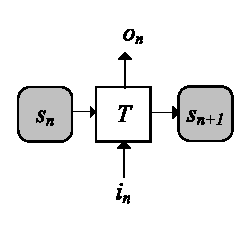
\includegraphics{mealy}
% \caption{Mealy finite state machine}
% \label{mealy}
% \end{figure}

The encoder is modeled by a finite state machine(FSM) $M=(\vec{s},\vec{i},\vec{o},T)$,
consisting of a state variable vector $\vec{s}$,
% an initial state $s_0\in S$,
an input variable vector $\vec{i}$,
% a finite set of configuration letters $C$,
an output variable vector $\vec{o}$,
and a transition function $T: [\![\vec{s}]\!]\times [\![\vec{i}]\!]\to [\![\vec{s}]\!]\times [\![\vec{o}]\!]$ 
that computes the next state and output variable vector from the current state and input variable vector.

% As shown in Figure \ref{mealy},
% as well as in the remainder of this paper,
% the state is represented as a gray round corner box,
% and the transition function $T$ is represented as a white rectangle.
The behavior of FSM $M$ can be reasoned by unrolling transition function for multiple steps.
The state variable $s\in\vec{s}$, input variable $i\in\vec{i}$ and output variable $o\in\vec{o}$ at the $n$-th step 
are respectively denoted as $s_n$, $i_n$ and $o_n$.
Furthermore,
the state, the input and the output variable vectors at the $n$-th step are respectively denoted as $\vec{s}_n$, $\vec{i}_n$ and $\vec{o}_n$.
% We further denote the sequence of state, input letter and output letter from the $n$-th to the $m$-th step respectively as $s_n^m$, $i_n^m$ and $o_n^m$.
A \textbf{path} is a state sequence $<\vec{s}_n,\dots,\vec{s}_m>$ with $\exists \vec{i}_j\vec{o}_j (\vec{s}_{j+1},\vec{o}_j)\equiv T(\vec{s}_j,\vec{i}_j)$ for all $n\le j< m$.
A \textbf{loop} is a path $<\vec{s}_n,\dots,\vec{s}_m>$ with $\vec{s}_n\equiv \vec{s}_m$.





\section{The software architecture}\label{sec_arch}
The CompSyn tool is implemented in the OCaml language.
Its architecture is shown in Figure \ref{fig_arch},
which comprises the following major components:

\begin{figure}[b]
\centering
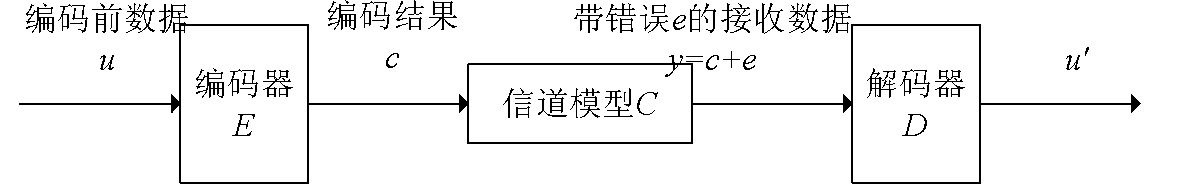
\includegraphics[width=0.8\textwidth]{arch}
\caption{The architecture of CompSyn}
\label{fig_arch}
\end{figure}

\subsection{Syntax analyzer}



\subsection{AIG manager}

This AIG manager represents a circuit with an array.
% The access time of the array type in OCaml language is much faster than that of the list type,
% because it can be accessed directly with an integer index,
% while the access time of the list type is propositional to the list's length.
Elements of this array are of the following types:

\begin{enumerate}
\item TRUE: A logical constant true without parameter.
\item FALSE: A logical constant false without parameter.
\item VARIABLE: A node with an integer parameter,
which is this variable's encoding number.
\item INVERTER: An inverter with an integer parameter,
which refers to the index of the element that drives this inverter.
\item BUFFER:   A non-inverted buffer with an integer parameter,
which refers to the index of the element that drives this buffer.
\item AND: A two-input AND gate with two integer parameters that refer to the indexes of the elements that drive this AND gate.
\end{enumerate}

This AIG manager provides some procedures to manipulate the circuit represented in AIG,
such as removing redundant elements,
propagating constance,
and translating an AIG circuit to CNF formula.

\subsection{CNF manager}

This manager takes care of all CNF formulas generated by the syntax analyzer,
unrolled transition relations used to determine the existence of the decoder,
the formulas used to generate Craig interpolant,
and the formulas used to test functional dependency 

The set of clauses of a CNF formula is stored in an OCaml list,
while each element of this list is another list that stores this clause's literal set.
The reasons for using list are that the clauses in a CNF formula do not need to be randomly accessed,
and the list type provides the flexibility to increase the size of the formula dynamically.

\subsection{The SAT solver interface and the SAT solver}

The SAT solver used here is the minisat solver v1.14 
This solver provides the ability to generate a proof for an unsatisfiable formula,
which can be analyzed to generate a Craig interpolant.

The proof generated by the minisat solver often includes most of the clauses appearing in the original formula,
which causes huge runtime overhead in generating Craig interpolant.
To reduce this overhead,
the minisat solver is modified to minimize the proof,
by removing those redundant clauses.

The OCaml to C interface that links CompSyn and minisat together is MiniSat-ocaml  developed by Flavio Lerda.
However,
one of its major shortcomings is that it does not provide the ability to read back the proof from the minisat solver.
Hence,
such a procedure is added.

The other major shortcoming of this interface is that it only provides a procedure to allocate new variables one by one.
As the overhead of calling C procedure from OCaml is very high,
this will lead to very large runtime overhead for large formulas.
To reduce this overhead,
a new procedure that allocates all new variables in one calling is added.

\subsection{The Craig interpolant generator and the BDD interface}

The Craig interpolant generator works on the proof return from the minisat solver,
and generates the interpolant in AIG form.
One shortcoming of our Craig interpolant generator,
which is also shared by other implementations of the same algorithm 
is that the generated interpolant contains lots of redundant gates.

To remove these redundant gates,
the CUDD package is invoked to generate a canonical representation of the interpolant.
The OCaml to C interface that links CUDD to CompSyn is taken from Blast model checker

After the simplification,
the BDD is converted back to a much more compact AIG by enumerating all cubes of this BDD.

\section{An overview of the synthesis mode}\label{sec_syn}

The overall flow of the synthesis mode is shown in Figure \ref{fig_halting}.
The loop iteratively increases the window size and unrolls the transition relation on that window.
Each iteration determines the decoder's existence by checking the $PC$ condition,
and determine the decoder's nonexistence by checking the $LN$ condition.
These two conditions will be introduced intuitively in the following subsections.

\begin{figure}[t]
\centering
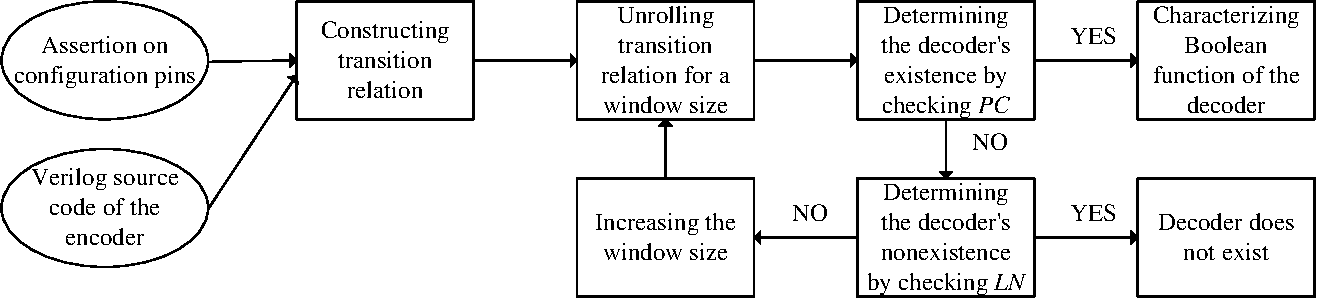
\includegraphics[width=\textwidth]{halting}
\caption{The flow of the synthesis mode}
\label{fig_halting}
\end{figure}

\subsection{Constructing transition relation}

This step takes two inputs,
one is the encoder's Verilog source code,
the other is the assertion on the encoder's configuration pins.
Normally,
an encoder has several modes,
each of which corresponds to a non-overlapped state set:

One of the most important modes is the working mode,
in which the encoder encodes its input.
Hence,
the encoder's input can be determined by its output,
which leads to the existence of its decoder.

On the other hand,
the encoder still has many other non-working modes,
such as the testing and sleep mode,
in which the encoder processes test commands or does nothing,
respectively.
Therefore,
in these modes,
the encoder's input cannot be determined by its output,
which leads to the nonexistence of its decoder.

Therefore,
the user needs to specify an assertion here to constrain the correct value of the encoder's configuration pins,
such that the encoder can be put in the correct working modes.


% \begin{figure}[t]
% \begin{center}
% 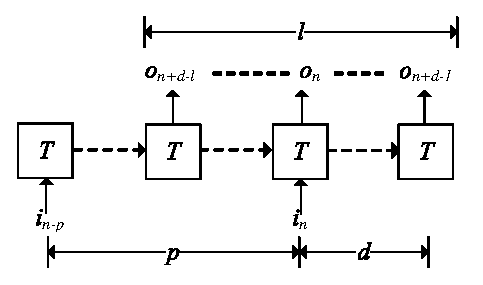
\includegraphics{t1}
% \end{center}
% \caption{The parameterized complementary condition}
%   \label{t1}
% \end{figure}
%
% \begin{figure}[b]
% \begin{center}
% 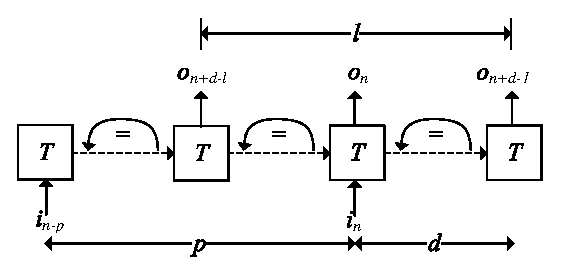
\includegraphics{doubleloop}
% \end{center}
% \caption{The loop-like non-complementary condition}
%   \label{doubleloop}
% \end{figure}

\subsection{Unrolling the transition relation and checking $PC$}

\begin{figure}[t]
\begin{center}
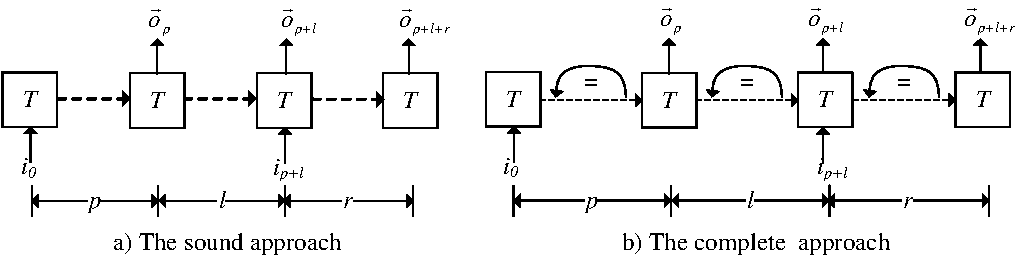
\includegraphics[width=\textwidth]{pc}
\end{center}
\caption{The $PC$ condition}
  \label{fig_pc}
\end{figure}

$PC$ is the abbreviation of Parameterized Complementary Condition defined in ,
which is used to determine the existence of the decoder.
Its meaning is intuitively shown in Figure \ref{fig_pc},
where $T$ is the encoder's transition relation constructed in the previous step,
while $i_n$ and $o_n$ are the input and output letter,
respectively,
and $p$, $d$, and $l$ are the lengths of the unfolded transition relation,
which are also called \textbf{the window size}.

This figure,
and therefore $PC$,
indicates that the decoder exists if and only if there exists $p$, $d$, and $l$,
such that the output sequence $<o_{n+d-l},\dots,o_{n+d-1}>$ can uniquely determine the input letter $i_n$.
In other words,
there does not exist two different input letters $i_n$ and $i_n'$ that can be recovered from the same output sequence $<o_{n+d-l},\dots,o_{n+d-1}>$.

This condition can be encoded into a SAT instance and solved with the minisat solver 
If the result is unsatisfiable,
then the decoder exists;
otherwise,
the decoder does not exist for this particular value of $p$, $d$, and $l$.
CompSyn needs to check $LN$ or increase the window size.

\subsection{Checking $LN$}
\begin{figure}[t]
\begin{center}
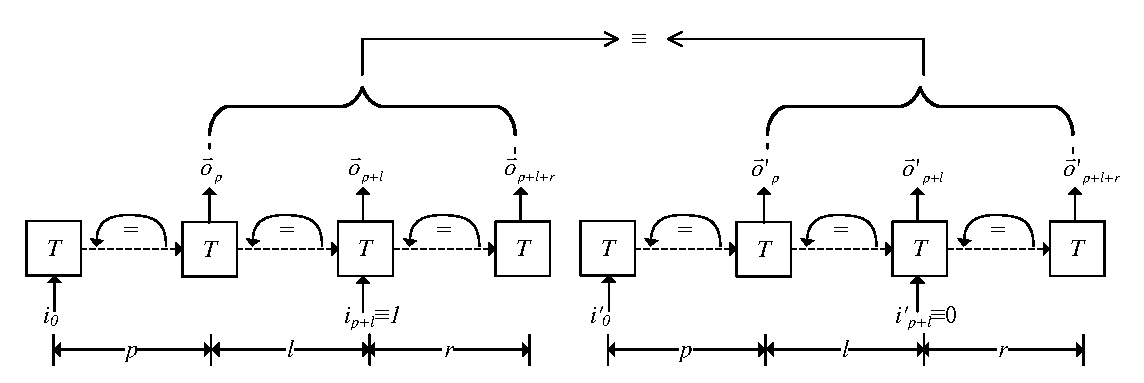
\includegraphics[width=\textwidth]{ln}
\end{center}
\caption{The $LN$ condition}
  \label{fig_ln}
\end{figure}

In addition to the $PC$ mentioned in the last subsection,
another condition $LN$ had been defined in to determine the nonexistence of the decoder.
Its meaning is intuitively shown in Figure \ref{fig_ln},
indicating that the decoder does not exist if and only if there exists $p$, $d$, and $l$,
such that the output sequence $<o_{n+d-l},\dots,o_{n+d-1}>$ can \textbf{NOT} uniquely determine the input letter $i_n$,
and there are three loops on state sequences $<s_{n-p},\dots,s_{n+d-l}>$,$<s_{n+d-l+1},\dots,s_n>$, and $<s_{n+1},\dots,s_{n+d}>$.

This condition can be encoded into a SAT instance,
and solved with the minisat solver 
If this SAT instance is satisfiable,
then the nonexistence of the decoder for all those longer paths can be proved by unfolding these loops.
Otherwise,
the window size will be increased and a new iteration will begin.
We have proven inthat the loop between $LN$ and $PC$ will eventually terminate.



\subsection{Characterizing the Boolean function of the decoder}

If the $PC$ checking succeeds,
then there exists a function that maps the output sequence $<o_{n+d-l},\dots,o_{n+d-1}>$ back to the input letter $i_n$.
This function can be characterized from the Boolean relation shown in Figure \ref{fig_pc},
with the ALLSAT algorithm proposed in 

Recently,
Liu et al.  proposed a much faster algorithm based on Craig interpolant to characterize this function.
The timing and area of the decoder generated by it is comparable to our ALLSAT algorithm.

This algorithm had also been implemented in CompSyn.
%whose major idea is shown intuitively in Figure \ref{fig_craig}.
To simplify the presentation,
we denote $i_n$ as $Y$,
the $j$-th bit of $Y$ as $Y^{j}$,
and $<o_{n+d-l},\dots,o_{n+d-1}>$ as $X$.
$R(X,Y)$ is the Boolean relation shown in Figure \ref{fig_pc},
which succeeds in checking $PC$.
As $R$ can uniquely determine the value of $Y$ from $X$,
a Craig interpolant of $R(X,Y)\wedge Y^{j}\equiv 1$ with respect to $R(X,Y')\wedge Y'^{j} \equiv 0$ can be generated.
This Craig interpolant is exactly the Boolean function that computes the $j$-th bit of $Y$ from $X$.
%\begin{figure}[b]
%\begin{center}
%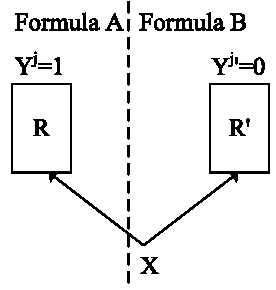
\includegraphics[width=0.15\textwidth]{craig}
%\end{center}
%\caption{Characterizing the Boolean function of the decoder with Craig interpolant}
%  \label{fig_craig}
%\end{figure}



\section{An overview of the inferring mode}\label{sec_infer}
To manually specify an assertion,
the user must read extensive documentation
and often perform laborious trial-and-error process.
This is why we develop the inferring mode that infers the assertion automatically.

The flow of the inferring mode is shown in Figure \ref{fig_infer}.
It is similar to Figure \ref{fig_halting},
with some new steps in gray color.
The assertion can be automatically inferred in this mode,
so the user does not need to specify it here.

One major difference while compared to the synthesis mode is the inner loop on the Checking $LN$ step.
Because the Checking $LN$ step can find out a configuration pin value that leads to the decoder's nonexistence,
a new step is inserted after it to remove all such values,
to ensure all remained configuration pin values have corresponding decoders.

The other major difference is the addition of two steps after the outer loop.
Because the inferred assertion actually includes multiple configuration pin values,
there may simultaneously exist multiple decoders.
Therefore,
a new step is inserted to discover all of them,
and another step is inserted to infer a precondition formula for each decoder,
which represents the set of configuration values that can lead to this decoder's existence.

\begin{figure}[t]
\centering
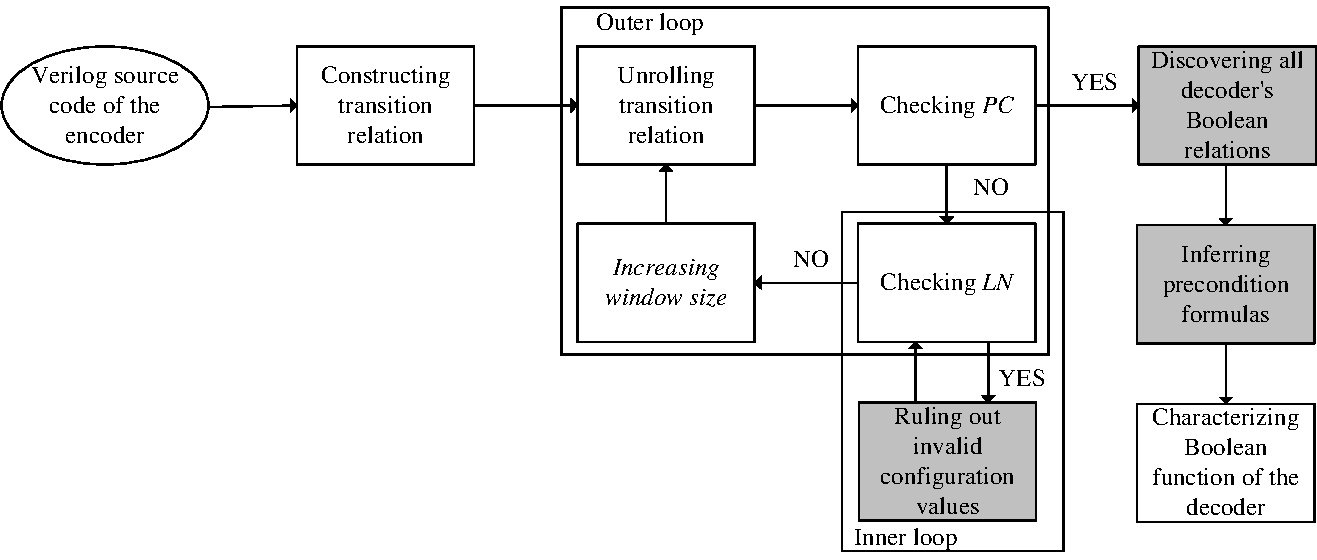
\includegraphics[width=\textwidth]{infer}
\caption{The flow of the inferring mode}
\label{fig_infer}
\end{figure}


\subsection{Ruling out invalid configuration values}

If the $LN$ checking succeeds,
an invalid configuration value that leads to the nonexistence of the decoder can be obtained from the  minisatolver's satisfying assignment.
We can simply rule out this invalid configuration value and return to the previous step to check $LN$ again.
However,
to reduce the runtime overhead,
an algorithm has been proposed to enlarge this value to a larger set of invalid configuration values with Craig interpolant ,
such that they can be rule out altogether.
\begin{figure}[t]
\centering
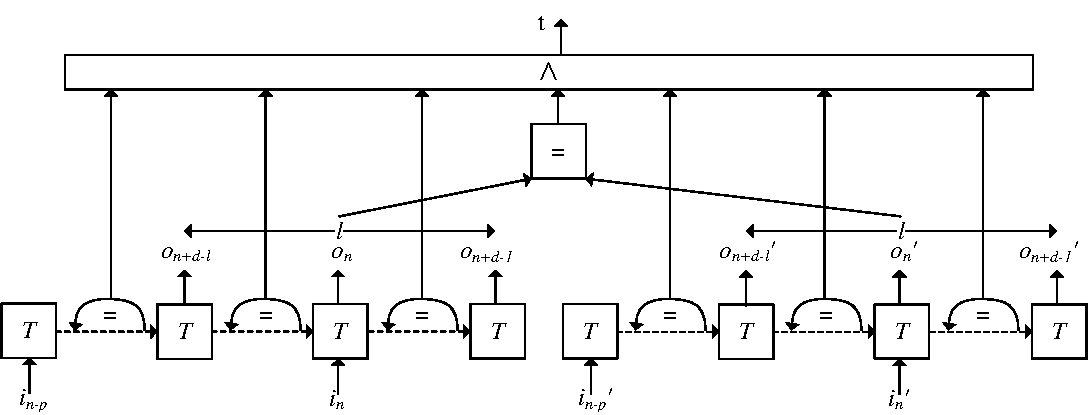
\includegraphics[width=\textwidth]{lninfer}
\caption{Enlarging the invalid configuration value with Craig interpolant}
\label{fig_lninfer}
\end{figure}

The formula used in enlarging is shown in Figure \ref{fig_lninfer}.
It is very similar to that of Figure \ref{fig_ln},
except that the existence of the six loops and the equality of the two output sequences are conjuncted together to generate a new Boolean variable $t$.
By assigning all $i_n$'s and $i_n'$'s satisfying assignment to Figure \ref{fig_lninfer},
this formula can be transformed into a new formula $F(c,t)$,
which defines a circuit,
whose input is the configuration value $c$,
and output is $t$.

The Boolean function of this circuit can be characterized by generating the Craig interpolant of $F(c,1)$ with respect to $F(c,0)$.
Thus,
this Boolean function is exactly the enlarged set of invalid configuration values.


The inner loop between this step and the Checking $LN$ step will eventually terminate after such invalid configuration values are all ruled out.
Then,
the window size is increased to check $PC$ again.



We have proven in  that the outer loop between $LN$ and $PC$ will eventually terminate.
Assume that the set of all configuration values ruled out is $NA$,
then the final inferred assertion is $\wedge_{na\in NA}\neg na$.

\subsection{Discovering all decoders' Boolean relations}

\begin{figure}[b]
\centering
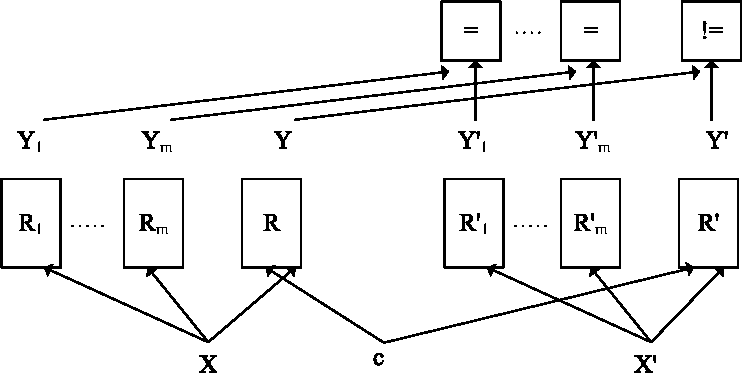
\includegraphics[width=0.7\textwidth]{fdtest_dec}
\caption{The SAT instance that discovers all decoders}
\label{fig_fdtest_dec}
\end{figure}

The final inferred assertion is a formula that actually contains many different configuration values.
This means that multiple decoders may exist simultaneously for this inferred assertion.
Thus,
we need to find out the set of all decoders' step by step.

We denote $i_n$ as $Y$,
$<o_{n+d-l},\dots,o_{n+d-1}>$ as $X$,
and the configuration value as $c$.
Then $R(c,X,Y)$ is the Boolean relation shown in Figure \ref{fig_pc} that succeeds in checking $PC$.

Assume $\{R_1,\dots,R_{m}\}$ is a set of decoders' Boolean relations that has already been discovered.
To test whether all decoders have already been discovered,
the SAT instance shown in Figure \ref{fig_fdtest_dec} is constructed based on functional dependency .

% In Figure \ref{fig_fdtest_dec},


According to ,
if this SAT instance is unsatisfiable,
then $Y$ can be uniquely determined by $\{Y_1,\dots,Y_m\}$,
which means all decoders have been discovered.
Otherwise,
a new decoder's Boolean relation can be discovered by assigning the satisfying assignment of $c$ to $R$.

A new round of functional dependency test will be performed again,
until no more decoder can be discovered.
Subsequently,
these Boolean relations will be used to characterize their corresponding decoders' Boolean functions,
with the ALLSAT algorithm .

\subsection{Inferring precondition formulas}
\begin{figure}[b]
\centering
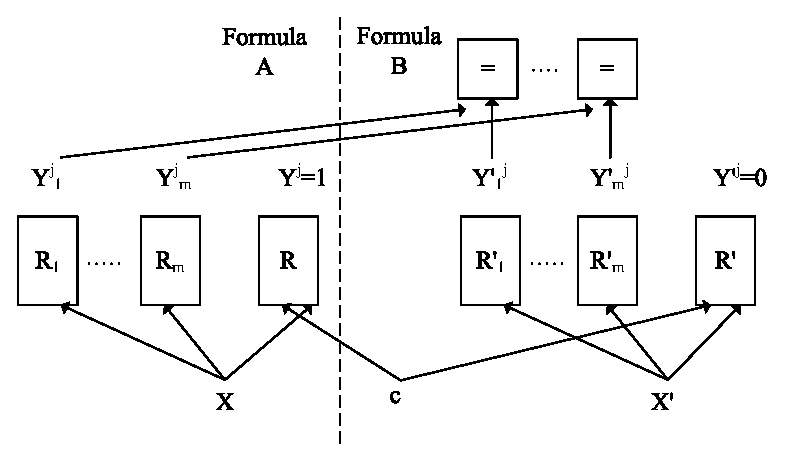
\includegraphics[width=0.7\textwidth]{fdtest_infer}
\caption{The SAT instance that infers precondition formulas}
\label{fig_fdtest_infer}
\end{figure}

Assume that $\{R_1,\dots,R_{m}\}$ is the set of all decoders' Boolean relations discovered in the last step,
and $\{IA_1,\dots,IA_{m}\}$ is their corresponding set of configuration letters.
To help the user determine which $R_i$ in $\{R_1,\dots,R_{m}\}$ is the correct decoder,
each $IA_i$ in $\{IA_1,\dots,IA_{m}\}$ must be characterized.

Assume $Y$ and all $Y_i$ in Figure \ref{fig_fdtest_dec} are vectors of the same length $v$,
and their $j$-th bit are $Y^{j}$ and $Y_i^{j}$,respectively.
If the precondition formulas $IA^j_i$ for the $j$-th bit of $IA_i$ can be characterized,
then $IA_i$ can be defined as $\bigwedge _{j=0}^{v-1} IA^j_i$.

To achieve this goal,
the unsatisfiable SAT instance shown in Figure \ref{fig_fdtest_infer} is constructed.
This SAT instance is very similar to that of Figure \ref{fig_fdtest_dec},
except that only the $j$-th bit is constrained.
Therefore it is unsatisfiable.
% which represents a functional dependency problem .
As the set of common variables between formula $A$ and $B$ is $\{c, Y_1^j, \dots, Y_m^j\}$,
the generated interpolant of $A$ with respect to $B$ is a function $F(c,Y_1^j, \dots, Y_m^j)$ that computes the value of $Y^j$.
By setting the value of $Y_i^j$ to 1 and all other $\{Y_k^j|k\ne i\}$ to 0 in $F(c,Y_1^j, \dots, Y_m^j)$,
we can obtain the formula $IA^j_i$.
%\begin{figure}[t]
%\centering
%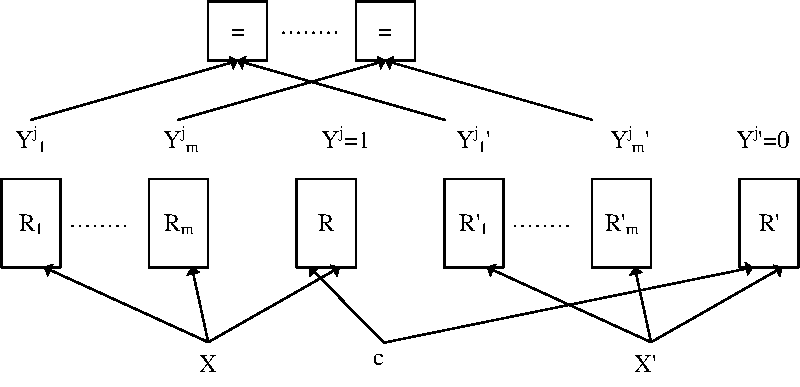
\includegraphics[width=0.75\textwidth]{fdtest_simple}
%\caption{The SAT instance that infers precondition formulas}
%\label{fig_fdtest_simple}
%\end{figure}



\section{Experimental results}\label{sec_exp}
\subsection{The usage model}
All these steps mentioned above are connected together by the standard make tool in Linux.
To use the synthesis mode,
the user needs to run the command "make halting" under the bash shell in the benchmark directory.
To use the inferring mode,
the user needs to run the command "make infer\_multidec\_not\_charfirst \_nowall".

\subsection{Benchmarks}
The benchmarks used in the experiments include several complex encoders from industrial projects,
\begin{enumerate}
\item A XGXS encoder compliant to clause 48 of IEEE-802.3ae 2002 standard .
\item A XFI encoder compliant to clause 49 of the same IEEE standard.
\item A 66-bit scrambler used to ensure
that a data sequence has sufficient 0-1 transitions,
so that it can run through a high-speed
noisy serial transmission channel.
\item A PCI-E physical coding module .
\item The Ethernet module of Sun's OpenSparc T2 processor.
\end{enumerate}

The profiles of these benchmarks are shown in Table \ref{tab_benchmark}.
Some of these large benchmarks have more than 1000 lines of source code,
while the XFI encoder has more than 100 state variables and configuration pins.


\begin{table}[t]
\centering
\caption{Information on Benchmarks}
\begin{tabular}{|c|c|c|c|c|c|}
\hline
&XGXS&XFI&scrambler&PCIE&T2 Ethernet\\\hline\hline
Line number&&&&&\\
of verilog&214&466&24&1139&1073\\
source code&&&&&\\\hline
\#state variables&15&135&58&22&48\\\hline
Data path width&8&64&66&10&10\\\hline
\end{tabular}\label{tab_benchmark}
\end{table}

\subsection{The experimental result of the synthesis mode}
\begin{table}[t]
\centering
\caption{Experimental results on the correct and incorrect encoders}
\begin{tabular}{|c|c|c|c|c|c|c|}
\hline
&                                        &XGXS     &XFI       &scrambler     &PCI-E    &T2 Ethernet\\ \hline\hline
% &Time to ch-                           &&&&&\\
% 
% &$d,p,l$                                 &1,1,1    &0,3,2     &0,2,2     &2,1,1   &4,1,1         \\ \hline\hline
For &Time to check the                         &&&&&\\
correct&decoder's existence(sec)                      &0.29     &17.86     &2.67      &0.47    &29.64\\\cline{2-7}
%      &improve \%                         &72.64    &74.67     &53.48     &80.42   &55.34 \\\cline{2-7}
encoder&$d,p,l$                                 &1,2,1    &0,3,2     &0,2,2     &2,2,1   &4,4,1          \\ \hline\hline
For&Time to check the                          &&&&&\\
incorrect&decoder's existence(sec)             &0.16     &7.59     &1.17      &0.33    &2.19\\
encoder&                        &&&&&\\\hline

\end{tabular}\label{tab_prodes}
\end{table}

According to Table \ref{tab_prodes} and ,
when given the assertion,
%no matter correct or not,
the synthesis mode can determine the existence of the decoders within 40 seconds,
and builds the decoders within 10 seconds with an algorithm similar to that of Liu et al. .

Moreover,
we inserted some bugs into these encoders,
which generated the same output letter for two different input letters.
CompSyn successfully detected all these bugs within 10 seconds.

\subsection{The experimental result of the inferring mode}
\begin{table}[b]
\centering
\caption{Experimental Results of the inferring mode}
\begin{tabular}{|c|c|c|c|c|c|c|}
\hline
                                        &XGXS     &XFI       &scrambler     &PCI-E    &T2 Ethernet\\\hline\hline
Config                 &&&&&\\
pin number                              &3        &120       &1             &16      &26\\\hline
Runtime                                 &3.83     &3841.34   &18.73         &8.51    &1791.22      \\\hline
$d,p,l$                                 &1,5,1    &0,5,2     &0,4,2         &2,5,1   &4,5,1          \\ \hline
Number of                               &&&&&          \\
decoders                                &1        &2         &2             &1       &1          \\ \hline
\end{tabular}\label{tab_res}
\end{table}

According to Table 	\ref{tab_res},
when the assertions are not known,
the inferring mode can infer assertions, generate decoders and infer these decoders' precondition formulas within 4000 seconds.

The set of inferred assertions are shown below:

\textbf{For XGXS}:
\texttt{( ( !bad\_code ) )}

\textbf{For XFI}:
\texttt{( ( TEST\_MODE ) | ( !TEST\_MODE \& RESET ) | ( !TEST\_MODE \& !RESET \& DATA\_VALID ) )}

\textbf{For scrambler}:
\texttt{True}

\textbf{For PCI-E}:
\texttt{( ( !TXELECIDLE \& CNTL\_TXEnable\_P0 \& CNTL\_RESETN\_P0 \& !CNTL\_Loopback\_P0 ) )}

\textbf{For T2 ethernet}:
\texttt{( ( link\_up\_loc \& !reset\_tx \& !txd\_sel[1] \& !jitt er\_study\_pci[1] \& !txd\_sel[0] \& !jitter\_study\_pci[0] ) | ( !link\_up\_l oc \& !reset\_tx \& !txd\_sel[1] \& tx\_enc\_conf\_sel[3] \& tx\_enc\_conf\_sel[2] \& !jitter\_study\_pci[1] \& !txd\_sel[0] \& !jitter\_study\_pci[0] ) | ( !l ink\_up\_loc \& !reset\_tx \& !txd\_sel[1] \& tx\_enc\_conf\_sel[3] \& !tx\_enc\_conf \_sel[2] \& tx\_enc\_conf\_sel[1] \& !jitter\_study\_pci[1] \& !txd\_sel[0] \& !ji tter\_study\_pci[0] ) | ( !link\_up\_loc \& !reset\_tx \& !txd\_sel[1] \& !tx\_ enc\_conf\_sel[3] \& !tx\_enc\_conf\_sel[2] \& tx\_enc\_conf\_sel[1] \& !jitter\_ study\_pci[1] \& !txd\_sel[0] \& !jitter\_study\_pci[0] \& tx\_enc\_conf\_sel[0] ) )}

Moreover,
only two out of the five benchmarks have two decoders,
while the other three have only one decoder.
This means that,
in most cases,
our algorithm generates only one decoder.
For other cases with multiple decoders,
the user needs to inspect the inferred precondition formulas to select the correct one.

For the two decoders of scrambler,
their corresponding precondition formulas are $reset$ and $!reset$.
By inspecting the Verilog source code of scrambler,
we found that the $reset$ is used to reset the scrambler when it is $True$.
Thus,
the scrambler encoder will work in normal mode when $reset$ is $False$.
Therefore,
the second decoder is the correct one.
And the dynamic simulation had confirmed its correctness.


For the two decoders of the most complex XFI encoder ,
their corresponding precondition formulas are $RESET~\& !TEST\_MODE~\&~!DATA\_VALID$ and $!RESET~\&~!TEST\_MODE~\&~DATA\_VALID$.
The only differences between them are the value of $RESET$ and $DATA\_VALID$.
By inspecting the Verilog source code of XFI,
we found that the $RESET$ is used to reset the XFI encoder when it is $True$,
and $DATA\_VALID$ means that the input data is valid when it is $True$.
So,
the XFI encoder will work in normal mode when $RESET$ is $False$ and $DATA\_VALID$ is $True$.
Therefore,
the second decoder is the correct one.
The dynamic simulation had also confirmed its correctness.

In this process,
the user only needs to inspect the meaning of two configuration pins,
instead of all 120 configuration pins of the XFI encoder.
In this way,
the human effort in specifying assertion and selecting the correct decoder is significantly reduced.

\section{Conclusions}\label{sec_conclude}
The CompSyn tool can infer correct assertions and generate decoder circuits for several complex encoders.
Furthermore,
it can significantly reduce the human effort in specifying assertion and selecting the correct decoder.


% \section*{Acknowledgment}
% The authors would like to thank the anonymous reviewers for their hard work.

% This work was funded by Projects 60603088 and 61070132 supported by National Natural Science Foundation of China.


\bibliographystyle{abbrv}
\bibliography{ssy}


% \begin{thebibliography}{4}
% 
% \end{thebibliography}



\end{document}
